\HeaderQuote{Read the directions and directly you will be directed in the right direction.}{Doorknob} 

\chapter{Scheduling}\label{ch:scheduling}
\FirstSentence{S}{cheduling problems}, which occur frequently in practice, are a category within combinatorial optimisation problems. 
A subclass of scheduling problems is the \jsp\ scheduling problem (\JSP), which 
is widely studied in operations research. 
\Jsp\ deals with the allocation of tasks of competing resources where its goal is to optimise a single or multiple objectives. 
\Jsp's analogy is from manufacturing industry where a set of jobs are broken down into tasks that must be processed on several machines in a workshop. 
Furthermore, its formulation can be applied on a wide variety of practical problems in real-life applications which involve decision making, therefore its problem-solving capabilities has a high impact on many manufacturing organisations. % Gefa dæmi?

Deterministic \JSP\ is the most \emph{general} case for classical scheduling problems \citep{Jain99}. 
Many other scheduling problems can be reformulated as \JSP. 
For instance, the \textit{travelling salesman problem} can be contrived as \jsp
\begin{enumerate*}[label={{}}]
    \item with the salesman as a single machine in use 
    \item the cities to be visited are the jobs to be processed
\end{enumerate*}
Moreover, the general form of \JSP\ assumes that each job can have its own 
distinctive flow pattern through the machines, which is independent of the 
other jobs. 
In the case where all jobs share the same permutation route, \jsp\ is reduced 
to a \fsp\ scheduling problem (\FSP) \citep{Guinet1998,Tay08}. 
Therefore, without loss of generality, this dissertation is structured around 
\JSP. 

\emph{Remark:} Throughout the dissertation the \FSP\ variation will \emph{not} 
be a commonly used permutation \fsp\ (P\FSP) from the literature, which has 
the added constraints of not allowing any jobs to pass one another.
Here, the jobs have to be processed in the same machine order, however, 
machines do not necessarily need to process jobs in the same order, as is 
implied in P\FSP.


\section{\Jsp\ scheduling problem}
\Jsp\ considered for this dissertation is when $n$ jobs, 
$\mathcal{J}=\{J_j\}_{j=1}^n$, are scheduled on a finite set, 
$\mathcal{M}=\{M_a\}_{a=1}^m$, of $m$ machines, subject to the constraint that 
each job $J_j$ must follow a predefined machine order (a chain or sequence of 
$m$ operations, $\vsigma_j=[\sigma_{j1},\sigma_{j2},\dotsc,\sigma_{jm}]$) and 
that a machine can handle at most one job at a time. 
The objective is to schedule jobs in such a manner as to minimise the maximum completion times for all tasks, which is also known as the makespan, $C_{\max}$. A common notion for this family of scheduling problems, i.e., a $m$ machine \JSP\ w.r.t. minimising makespan, is $Jm||C_{\max}$ \citep[cf.][]{Pinedo08}. In addition, for \FSP\ w.r.t. minimising makespan the notation is $Fm||C_{\max}$. 
An additional constraint commonly considered are job release-dates and due-dates, and then the objective is generally minimising the maximum lateness, denoted $Jm||L_{\max}$, however, those  constraints will not be considered here. 

Henceforth, the index $j$ refers to a job $J_j\in\mathcal{J}$ while the index 
$a$ refers to a machine $M_a\in\mathcal{M}$. If a job requires a number of 
processing steps or operations, then the pair $(j,a)$ refers to the operation, 
i.e., processing the task of job $J_j$ on machine $M_a$. Moreover, index $k$ 
will denote the time step of the operation. Note that once an operation is 
started, it must be completed uninterrupted, i.e., pre-emption is not allowed. 
Moreover, there are no sequence dependent set-up times.

\section{Mathematical formulation}
For any given \JSP, which consists of $n$ jobs for $m$ machines, then each job $J_j$ has an indivisible operation time (or cost) on machine $M_a$, $p_{ja}$, which is assumed to be integral and finite. 
Starting time of job $J_j$ on machine $M_a$ is denoted $x_s(j,a)$ and its 
completion or end time is denoted $x_e(j,a)$ where, 
\begin{equation}  x_e(j,a):=x_s(j,a)+p_{ja} \end{equation} 
Each job $J_j$ has a specified processing order through the machines, it is a permutation vector, $\vsigma_j$, of $\{1,..,m\}$, representing a job $J_j$ can be processed on $M_{\vsigma_j(a)}$ only after it has been completely processed on $M_{\vsigma_j(a-1)}$, i.e.,
\begin{equation}\label{eq:permutation}
	x_s(j,\vsigma_j(a)) \geq x_e(j,\vsigma_j(a-1)) 
\end{equation}
for all $J_j\in\mathcal{J}$ and $a\in\{2,..,m\}$. 
Note, that each job can have its own distinctive flow pattern through the 
machines, which is independent of the other jobs. However, in the case that all 
jobs share the same permutation route, \JSP\ is reduced to a \FSP.

The disjunctive condition that each machine can handle at most one job at a time is the following,
\begin{equation}\label{eq:oneJobPerMac}
	x_s(j,a) \geq x_e(j',a) \quad\textrm{or}\quad x_s(j',a) \geq x_e(j,a)  
\end{equation}
for all $J_j,J_{j'}\in\mathcal{J},\; J_j\neq J_{j'}$ and $M_a\in\mathcal{M}$. 

The objective function is to minimise its maximum completion times for all tasks, commonly referred to as the makespan, $C_{\max}$, which is defined as follows,
\begin{equation}
	C_{\max} := 
	\max\condset{x_e(j,\vsigma_j(m))}{J_j\in\mathcal{J}}.\label{eq:makespan}
\end{equation} 
Clearly, w.r.t. minimum makespan, it is preferred that schedules are non-delay, 
i.e., the machines are not kept idle. The time in which machine $M_a$ is idle 
between consecutive jobs $J_j$ and $J_{j'}$ is called idle time, 
\begin{equation} s(a,j):=x_s(j,a)-x_e(j',a) \label{eq:slack}\end{equation}
where $J_j$ is the immediate successor of $J_{j'}$ on $M_a$. Although this is 
not a variable directly needed to construct a schedule for \JSP, it is a key 
attribute in order to measure the quality of the schedule. 

\section{Construction heuristics}\label{sec:CH}
Construction heuristics are designed in such a way that it limits the search space in a logical manner, respecting not to exclude the optimum. Here, the construction heuristic is to schedule the dispatches as closely together as possible, i.e., minimise the schedule's flow. 
More specifically, once an operation $(j,a)$ has been chosen from the job-list, 
$\mathcal{L}$, by some dispatching rule, it can placed immediately after (but 
not prior) $x_e(j,\vsigma_j(a-1))$ on machine $M_a$ due to constraint 
\cref{eq:permutation}. 
However, to guarantee that constraint \cref{eq:oneJobPerMac} is not violated, 
idle times $M_a$ are inspected, as they create flow time  which $J_j$ can 
occupy. Bearing in mind that $J_j$ release time is $x_e(j,\vsigma_j(a-1))$ one 
cannot implement \cref{eq:slack} directly, instead it has to be updated as 
follows,
\begin{eqnarray}
	\tilde{s}(a,j')&:=& x_s(j'',a)-\max\{x_e(j',a),\;x_e(j,\vsigma_j(a-1))\} % 
	%\textrm{ if } x_e(j,\vsigma_j(a-1)\geq x_e(j',a) 
\end{eqnarray}
for all already dispatched jobs $J_{j'},J_{j''}\in \mathcal{J}_a$ where $J_{j''}$ is $J_{j'}$ successor on $M_a$. Since pre-emption is not allowed, the only applicable slots are whose idle time can process the entire operation, i.e.,
\begin{eqnarray}
	\tilde{S}_{ja}&:=&\condset{J_{j'}\in \mathcal{J}_a}{\tilde{s}(a,j')\geq 
	p_{ja} }\label{eq:slots}.
\end{eqnarray} 
Now, there are several heuristic methods for selecting a slot from 
\cref{eq:slots}, e.g., if the main concern were to utilise the slot space, then 
choosing the slot with the smallest idle time would yield a closer-fitted 
schedule and leaving greater idle times undiminished for subsequent dispatches 
on $M_a$. However, dispatching $J_j$ in the first slot would result in its 
earliest possible release time, which would be beneficial for subsequent 
dispatches for $J_j$. Preliminary experiments favoured dispatching in the first 
(earliest) slot,\footnote{Preliminary experiments of 500 \JSP\ instances where 
inspected: First slot chosen could always achieve its known optimum by 
implementing the pseudo code in \cref{pseudo:constructJSP}, however, only 
$97\%$ of the instances when choosing the smallest slot.} and henceforth will 
be used throughout the dissertation.

\input{pseudocode/constructJSP.tex}

Note that the choice of slot is an intrinsic heuristic within the construction heuristic.
Construction heuristics are designed in such a manner that they limit the 
search space. Preferably without excluding the true optimum. The focus of this 
dissertation, however, is on learning the priority of the jobs on the job-list, 
for a fixed construction heuristic. Hence there are some problem instances in 
which the optimum makespan cannot be achieved due to the limitations of the 
schedule's construction heuristic of not being properly able to differentiate 
between which slot from $\tilde{S}_{ja}$ is the most effective. Instead, 
hopefully, the learning algorithm will be able to spot these problematic 
situations, should they arise, by inspecting the schedule's features and 
translate that into the jobs' priorities.

\section{Example}\label{sec:jsp:example}
There are many examples of \jsp\ for real-world application. 
However, for demonstration purposes, let's assume we are invited to the Mad 
Hatter's Tea Party in Wonderland (cf. \cref{fig:teaparty}). 
There are four guests attending, namely
\begin{enumerate*}[label={$J_\arabic*$)}, ref={{$J_\arabic*$}}, 
    itemjoin*={{, and our host }}]
    \item Alice\label{guest:alice}
    \item March Hare\label{guest:marchhare}
    \item Dormouse\label{guest:dormouse}
    \item Mad Hatter\label{guest:madhatter}
\end{enumerate*}
During these festivities, there are several things each member of the party has 
to perform, they all have to
\begin{enumerate*}[label={$M_\arabic*$)}]
    \item have wine or pour tea
    \item spread butter
    \item get a haircut
    \item check the time of the broken watch for themselves
    \item say what you mean, be it asking a riddle, telling a story, or singing 
    a song to the group
\end{enumerate*}
Our guests are very particular creatures, and would like to do these task in a 
very specific order, e.g., \ref{guest:marchhare} March Hare insists on doing 
them in alphabetical order. 
Moreover, they tend to be very absent-minded so each task takes them a 
different amount of time. 
Let's assume that their processing times and permutation ordering are given in 
\cref{tbl:example}.

\begin{figure}[b!]
    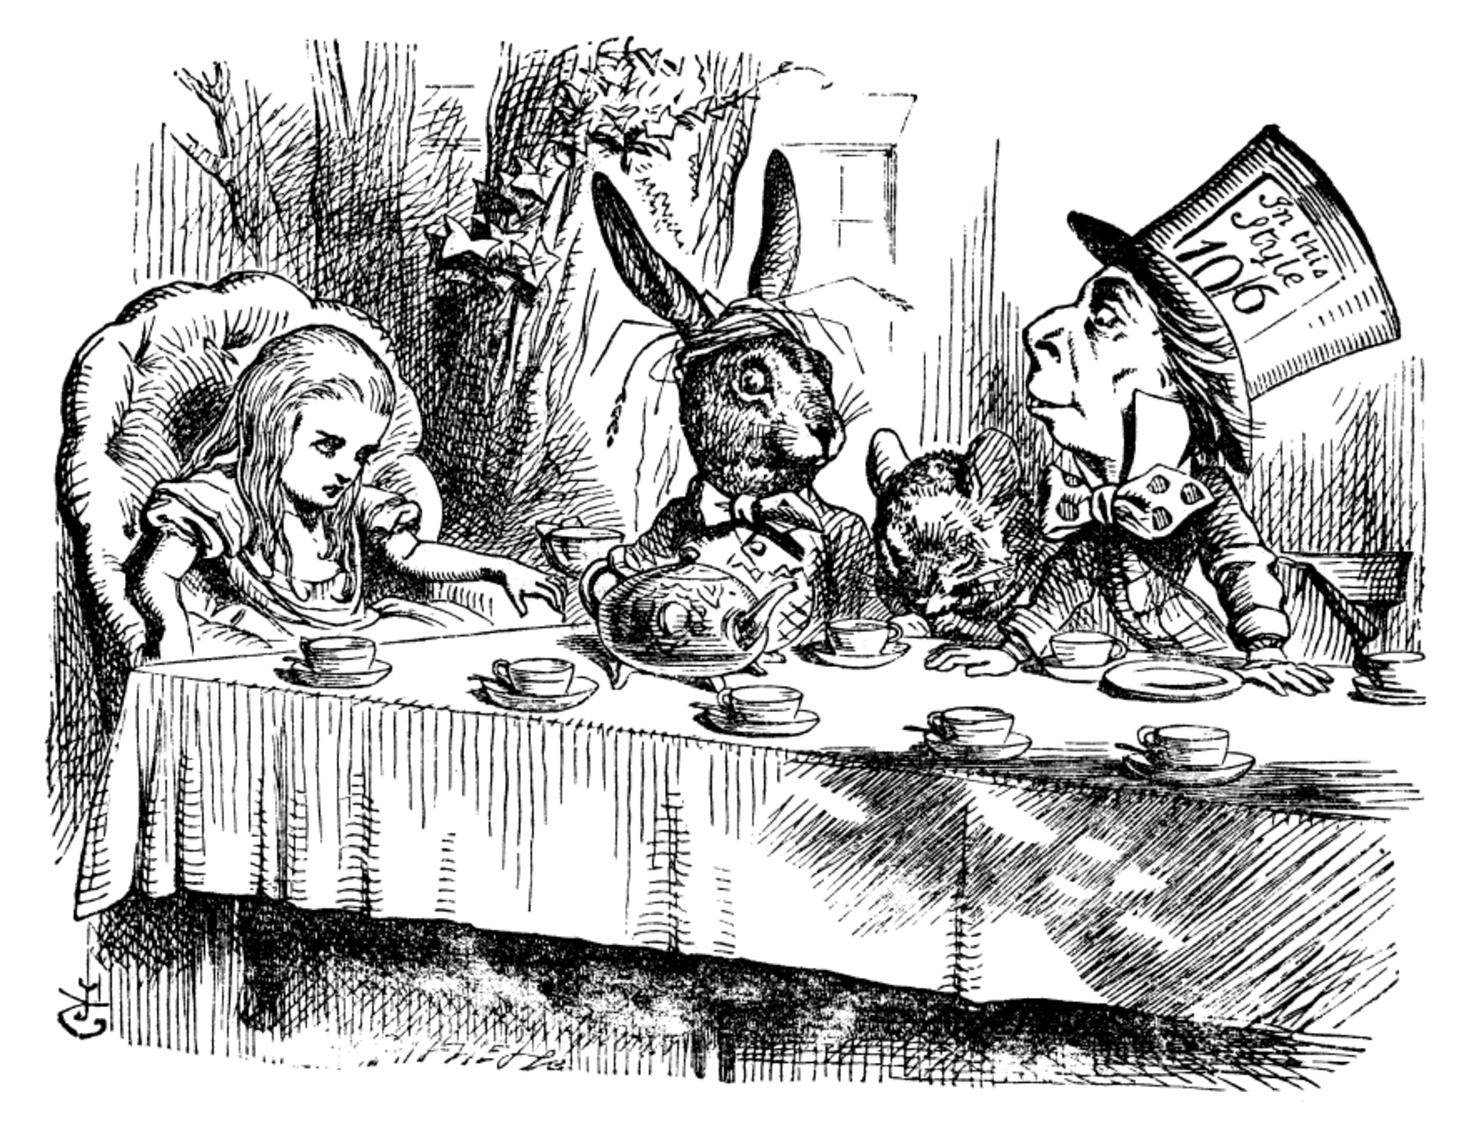
\includegraphics[width=\textwidth]{alice-mad-tea-party}
    \caption{The Mad Hatter's Tea Party, from Alice's Adventures in Wonderland 
        by \citet{alice}. Illustration by John Tenniel 
        (1820-1914).}\label{fig:teaparty}
\end{figure}

\begin{table}[h]\centering
%j.rnd.4x5.train.csv => instance problem.1
\caption{Example of $4\times5$ \JSP}\label{tbl:example}
\begin{tabular}{lc|ccccc|ccccc} \toprule
Guest & \multicolumn{1}{c}{Job} & \multicolumn{5}{c}{Machine ordering 
$\vsigma$} & \multicolumn{5}{c}{Processing times $\vec{p}$} \\ \midrule
%0 16 1 5 2 10 3 15 4 10 
Alice & \ref{guest:alice} & \textit{1} & \textit{2} & \textit{3} & \textit{4} & 
\textit{5} & 
\textit{26} & \textit{25} & \textit{40} & \textit{15} & \textit{42} \\
%0 18 1 16 2 36 3 68 4 44 
March Hare & \ref{guest:marchhare} & \textit{1} & \textbf{2} & 3 & 4 & 5 & 
\textit{18} & \textbf{86} & 86 & 68 & 84 \\
%4 20 3 9 2 3 1 33 0 96 
Dormouse & \ref{guest:dormouse} & \textit{1} & \textit{3} & \textbf{2} & 4 & 5 
& 
\textit{20} & \textbf{59} & \textit{23} & 33 & 96 \\
%4 40 3 7 1 15 5 13 2 80 
Mad Hatter & \ref{guest:madhatter} & \textit{4} & \textit{3} & \textbf{1} & 5 & 
2 & \textbf{40} & 47 & \textit{55} & \textit{13} & 99 
\\
\bottomrule
\end{tabular}
\end{table}

Unfortunately, Alice can't stay long. She must leave as soon as possible to 
play croquet with the Red Queen, 
and she mustn't be late for that very important date. Otherwise, it's off with 
someone's head! However, Alice, had a proper upbringing and won't leave the 
table until everyone has finished their tasks. 
How should the guests go about their tea-party, in order for Alice to be 
on-time?

Now we know that this fits perfectly to a six-job and five-machine \jsp\ 
problem, where our guests are the jobs and the tasks are the machines and our 
objective is to minimize the makespan, i.e., the release time for Alice. 
Let's assume we've come to the party, after 10 operations have already been 
made (i.e. the italic entries in \cref{tbl:example}), by using the following 
job sequence,
\begin{eqnarray}
	\vchi=\left[ J_4,J_2,J_3,J_3,J_1,J_1,J_1,J_1,J_1,J_4 \right]
\end{eqnarray}
hence the job-list is currently $\mathcal{L}^{(11)}=\{J_2,J_3,J_4\}$ (note that 
\ref{guest:alice}) Alice is quite anxious to leave, and has already completed 
everything) indicating the 3 potential jobs to be dispatched at step $k=11$ 
(i.e. denoted in bold in \cref{tbl:example}).
 
\Cref{fig:example:midway} illustrates the temporal partial schedule of the 
dispatching process as a Gantt-chart
\begin{enumerate*}
    \item numbers in the boxes represent the job identification $j$
    \item the width of the box illustrates the processing times for a given job 
    for a particular machine $M_a$ (on the vertical axis)
    \item the dashed boxes represent the resulting partial schedule for when a 
    particular job is scheduled next
    \item the current $C_{\max}$ is denoted with a dotted line    
\end{enumerate*}

\begin{figure}
    \includegraphics[width=\textwidth]{{example.gantt}.pdf}
    \caption[Gantt chart of a partial \JSP\ schedule]{Gantt chart of a partial 
        \JSP\ schedule after 10 dispatches: Solid and dashed boxes represent 
        $\vchi$ and $\mathcal{L}^{(11)}$, respectively. Current $C_{\max}$ 
        denoted 
        as dotted line.}
    \label{fig:example:midway}
\end{figure}

If the job with the shortest processing time were to be scheduled next, i.e., 
implementing the SPT heuristic, then $J_4$ would be dispatched. Similarly, for 
the LPT (largest processing time) heuristic then $J_2$ would be dispatched. 
Other DRs use features not directly observable from looking at the current 
partial schedule (but easy to keep record of), for example by assigning jobs 
with most or least total processing time remaining, i.e., MWR and LWR 
heuristics, who would yield $J_2$ and $J_4$, respectively.

To summarise, in order to create a schedule for \JSP, a construction heuristic 
is chosen with some DR to determine the priority of the jobs on the job-list, 
$\mathcal{L}$. \Cref{pseudo:constructJSP} outlines the pseudo code for the 
dispatching process of a \JSP\ problem instance.

Henceforth, a \emph{sequence} will refer to the sequential ordering of the 
dispatches of tasks to machines, i.e., $(j,a)$; the collective set of allocated 
tasks to machines, which is interpreted by its sequence, is referred to as a 
\emph{schedule}; a \emph{scheduling policy} will pertain to the manner in which 
the sequence is manufactured for an (near) optimal schedule: be it a SDR such 
as SPT or via evolutionary search, etc. 

\section{Single-based priority dispatching rules}\label{sec:SDR}
\emph{Dispatching rules} (DR) are of a construction heuristics, where one 
starts with an empty schedule and adds sequentially on one operation (or task) 
at a time. Namely, at each time step $k$, an operation is dispatched which has 
the highest priority of the job-list, 
\mbox{$\mathcal{L}^{(k)}\subset\mathcal{J}$}, i.e., the jobs who still have 
operations unassigned. If there is a tie, some other priority measure is used. 
However, let's assume that ties are broken at random. 

A \emph{single-based priority dispatching rule} (SDR), or simple priority 
dispatching rule, is a function of attributes, or features, of the jobs and/or 
machines of the schedule. The features can be constant or vary throughout the 
scheduling process. For instance, the priority may depend on job processing 
attributes, such as which job has, 
\begin{description}
	\item[Shortest immediate processing time (SPT)] \hfill \\
	greedy approach to finish shortest tasks first,  
	\item[Longest immediate processing time (LPT)] \hfill \\
	greedy approach to finish largest tasks first, 
	\item[Least work remaining (LWR)] \hfill \\
	whose intention is to complete jobs advanced in their pro\-gress, i.e., 
	minimising the job-list $\mathcal{L}$,
	\item[Most work remaining (MWR)] \hfill \\
	whose intention is to accelerate the processing of jobs that require a 
	great deal of work, yielding a balanced progress for all jobs during 
	dispatching, however, in-process inventory can be high.
\end{description}
These rules are the ones most commonly applied in the literature due to their simplicity and efficiency, %\citep[cf.][]{Haupt89,Panwalkar77}
therefore they will be referenced throughout the dissertation. 
However, there are many more available, e.g., randomly selecting an operation 
with equal possibility (RND); minimum slack time (MST); smallest slack per 
operation (S/OP); and using the aforementioned dispatching rules with 
predetermined weights. A survey of more than 100 of such rules are presented in 
\citet{Panwalkar77}, however, the reader is referred to an in-depth survey for 
SDRs by \citet{Haupt89}. 

%Haupt89:
%Among the rules with job processing information, SPT is the most known, the most applied, and yet one of the most efficient rules. In line with LPT, it requires the lowest information amount, since only operation data (not job data) from the local queue (not from other queues) are needed.
%LWR give preference to jobs the work completed of which is rather advanced. Thus, they can be regarded as value-oriented rules selecting jobs with a high fraction of their value added or cumulative value to their total value.
% The intent of MWR is to speed up jobs with large processing work resulting in a well-balanced work progress of all jobs, at the expense of a high volume of in-process inventory, while LWR tend to reduce the number of jobs in the shop.

To summarise, SDRs assign an index to each job of the job-list waiting to be 
scheduled, and are generally only based on few features and simple mathematical 
operations. 
Continuing with the example from \cref{sec:jsp:example}, the final schedules 
for these main SDRs (and a possible optimal schedule for reference) are 
depicted in \cref{fig:example:SDRs}.

\begin{figure}
    \includegraphics[width=\textwidth]{{example.gantt.SDRs}.pdf}
    \caption{SDRs applied to the example in \cref{sec:jsp:example}. 
    An optimal solution is shown in the lower right corner as a reference.}
    \label{fig:example:SDRs}
\end{figure}

%Haupt89:
%Among the rules with job processing information, SPT is the most known, the most applied, and yet one of the most efficient rules. In line with LPT, it requires the lowest information amount, since only operation data (not job data) from the local queue (not from other queues) are needed.
%LWR give preference to jobs the work completed of which is rather advanced. Thus, they can be regarded as value-oriented rules selecting jobs with a high fraction of their value added or cumulative value to their total value.
% The intent of MWR is to speed up jobs with large processing work resulting in a well-balanced work progress of all jobs, at the expense of a high volume of in-process inventory, while LWR tend to reduce the number of jobs in the shop.

\section{Features for \jsp}\label{sec:features}
A DR may need to perform a one-step look-ahead and observes features of the partial schedule to make a decision, for example by observing the resulting temporal makespan. These emanated observed features are sometimes referred to as an \emph{after-state} or \emph{post-decision state}. 

Features are used to grasp the essence of the current state of the schedule. Temporal scheduling features applied in this dissertation for a job $J_j$ to be dispatched on machine $M_a$ are given in \cref{tbl:features}. 
Note, from a job-oriented viewpoint, for a job already dispatched $J_j\in\mathcal{J}$ the corresponding set of machines now processed is $\mathcal{M}_j\subset\mathcal{M}$. Similarly from the machine-oriented viewpoint, $M_a\in\mathcal{M}$ with corresponding $\mathcal{J}_a\subset\mathcal{J}$. 

The features of particular interest were obtained from inspecting the aforementioned SDRs from \cref{sec:SDR}:  
\phiJobRelated\ and \phiMacRelated\ are job-related and machine-related attributes of the current schedule, respectively. 

Some features are directly observed from the partial schedule, such as the job- and machine-related features. 

Note that \phiLocalRelated\ are only based on the current step of the schedule, 
i.e., schedule's \emph{local features}, and might not give an accurate 
indication of how it will effect the schedule in the long run. Therefore, a set 
of features are needed to estimate the schedule's overall performance, referred 
to as its \emph{global features}. The approach here is to use well known SDRs, 
\phiSDRRelated, as a benchmark by retrieving what would the resulting 
$C_{\max}$ would be given if that SDR would be implemented from that point 
forward. Moreover, random completion of the partial schedule are implemented, 
here \phiRNDRelated\ corresponds to statics from 100 random roll-outs, which 
can be used to identify which features $\vphi$ are promising on a long-term 
basis.  

%All of the features vary throughout the scheduling process, w.r.t. operation 
%belonging to the same time step $k$, save for \phitotalProc\ which varies 
%between jobs; \phistep\ to keep track of features' evolution w.r.t. the 
%scheduling process; and \phiwrmTotal\ which is static for a given problem 
%instance, but used for normalising other features, such as work-remaining 
%based (\phiwrmJob\ and \phiwrmMac) or makespan-based (\phiGlobalRelated) ones.
%In addition, \phimac, is reported in order to distinguish which features are 
%in conflict with each other.

\begin{table} \centering 
	\caption[Feature space $\mathcal{F}$ for \JSP]{Feature space $\mathcal{F}$ for \JSP\ where job $J_j$ on machine $M_a$ given the resulting temporal schedule after dispatching $(j,a)$.}
	\label{tbl:features}
	 {\footnotesize

 \centering
 \renewcommand{\arraystretch}{1.5}
  \begin{tabular}{clll} %p{0.45\textwidth}|p{0.4\textwidth}|}
   \toprule
$\vphi$ & Feature description & Mathematical formulation& Shorthand\\ 
%\hline  \multicolumn{4}{c}{\textbf{Local features}}  \\
\midrule
 \multicolumn{4}{c}{\textbf{job related}}\\
  \phiproc & job processing time & $p_{ja}$&proc\\
  \phistartTime & job start-time  & $x_s(j,a)$ &startTime\\
  \phiendTime & job end-time & $x_f(j,a)$ &endTime\\
  \phiarrivalTime & job arrival time &$x_f(j,a-1)$ & arrival\\ 
  \phitotalProc & total processing time & $\sum_{a\in \mathcal{M}}p_{ja}$ & totalProc\\
  \phiwait & time job had to wait &$x_s(j,a)-x_f(j,a-1) $ & wait\\   
  \phiwrmJob & total work remaining for job & $\sum_{a'\in\mathcal{M}\setminus \mathcal{M}_{j}}p_{ja'}$ & wrmJob\\
  \phijobOps & number of assigned operations for job & $|\mathcal{M}_j|$ & jobOps\\ 
\midrule
 \multicolumn{4}{c}{\textbf{machine related}}\\
  \phimacFree & when machine is next free & $\max_{j'\in \mathcal{J}_a} 
  \{x_f(j',a)\}$& macFree\\
  \phiwrmMac & total work remaining for machine &$\sum_{j'\in\mathcal{J}\setminus \mathcal{J}_{a}}p_{j'a} $ & wrmMac\\
  \phimacOps & number of assigned operations for machine & $|\mathcal{J}_a|$ & macOps\\
\midrule
 \multicolumn{4}{c}{\textbf{flow related}}\\
  \phislotsReduced & change in idle time by assignment & $\Delta s(a,j)$& slotsReduced \\
  \phislots & total idle time for machine & $\sum_{j'\in \mathcal{J}_a}s(a,j')$ & slots\\
  \phislotsTotal & total idle time for all machines & $\sum_{a'\in \mathcal{M}}\sum_{j'\in \mathcal{J}_{a'}}s(a',j')$  & slotsTotal\\
\midrule
 \multicolumn{4}{c}{\textbf{current makespan related}}\\
  \phimakespan & current makespan & $\max_{(j',a')\in \mathcal{J} \times \mathcal{M}_{j'}}\{x_f(j',a')\}$ & makespan \\
\midrule
 \multicolumn{4}{c}{\textbf{final makespan related}}\\
\phiSPT & final makespan using SPT & $ C_{\max}|\text{DR}=\text{SPT}$ & SPT \\
\phiLPT & final makespan using LPT  & $ C_{\max}|\text{DR}=\text{LPT}$ & LPT \\
\phiLWR & final makespan using LWR & $ C_{\max}|\text{DR}=\text{LWR}$ & LWR \\
\phiMWR & final makespan using MWR & $ C_{\max}|\text{DR}=\text{MWR} $ & MWR \\
\phiRND & final makespan using 100 random rollouts & $ \{C_{\max}|\text{DR}=\text{RND}\}_{i=1}^{100}$ & RND \\  
   \bottomrule
  \end{tabular}
}
 %Feature description for job $J_j$ on machine $M_a$ given current temporal schedule, where the set of jobs already dispatched are $J\subset\mathcal{J}$ on corresponding set of machines $\mathcal{M}_j\subset\mathcal{M}$

\end{table}



\section{Composite dispatching rules}\label{sec:CDR}
\citet{Jayamohan04} showed that a careful combination of dispatching rules can perform significantly better. These are referred to as \emph{composite dispatching rules} (CDR), where the priority ranking is an expression of several SDRs. For instance, optimising \JSP\ w.r.t. $L_{max}$ for one machine\ \cite[see. chapter 14.2]{Pinedo08}, one can combine SDRs that are optimal for a different criteria of problem instances, which complement each other as a CDR, e.g., combining the SDRs 
WSPT (SPT weighted w.r.t. $\mathcal{J}$), ``which is optimal when all release dates and due dates are zero,'' 
and minimum slack first (MS), ``which is optimal when all due dates are sufficiently loose and spread out,'' 
one gets the CDR apparent tardiness cost which can work well on a broader set 
of problem instances than the original SDRs by themselves.

CDRs can deal with greater number of features and more complicated form, in 
short, CDR are a combination of several SDRs. For instance let $\pi$ be a CDR 
comprised of $d$ DRs (which could be SDR or another CDR), then the index $I$ 
for job $J_j$ using CDR is, 
\begin{equation}
	I_j^{\pi} = \sum_{i=1}^d w_i \cdot \pi_i(\vphi_j)
\end{equation}
where $w_i>0$ and $\sum_{i=0}^d w_i = 1$, then $w_i$ gives the \emph{weight} of 
the influence of $\pi_i$ to $\pi$. Note, 
each $\pi_i$ is a function of the job $J_j$'s feature state $\vphi_j$.

Generally the weights $\vec{w}$ are chosen by the algorithm designer a priori. 
A more sophisticated approach would to learn have the algorithm discover these 
weights autonomously, for instance via evolutionary search or preference-based 
imitation learning, to be discussed in \cref{ch:esmodels} and 
\cref{ch:prefmodels}, respectively.

\subsection*{Automated discovery of dispatching rules}
\citet{Monch13} stress the importance of automated discovery of DRs and named several of successful implementations in the field of semiconductor wafer fabrication facilities. 
However, \citeauthor{Monch13} note that this sort of investigation is still in its infancy and subject for future research.

A recent editorial of the state-of-the-art approaches in advanced dispatching rules for large-scale manufacturing systems by \citet{Chen13} points out that:
\begin{quote}
	[..] most traditional dispatching rules are based on historical data. With the emergence of data mining and on-line analytic processing, dispatching rules can now take predictive information into account.
\end{quote}
implying that there has not been much automation in the process of discovering new dispatching rules, which is the ultimate goal of this dissertation, i.e., automate creating optimisation heuristics for scheduling. 

With meta heuristics one can use existing DRs and use for example 
\emph{portfolio-based algorithm selection} \citep{Rice76,Gomes01}, either based 
on a single instance or class of instances \citep{Xu07} to determine which DR 
to choose from. 
Instead of optimising which algorithm to use under what data distributions, such as the case of portfolio algorithms, the approach taken in this dissertation is more similar to that of \emph{meta learning} \citep{Vilalta02} which is the study of how learning algorithms can be improved, i.e., exploiting their strengths and remedy their failings, in order for a better algorithm design. Thus creating an adaptable learning algorithm that dynamically finds the appropriate dispatching rule  to the data distribution at hand. 

\citet{Kalyanakrishnan11} point out that meta learning can be very fruitful in reinforcement learning, and in their experiments they discovered some key discriminants between competing algorithms for their particular problem instances, which provided them with a hybrid algorithm which combines the strengths of the algorithms.

\citet{Nguyen13} proposed a novel \emph{iterative dispatching rules} for \JSP\ 
which learns from completed schedules in order to iteratively improve new ones. 
At each dispatching step, the method can utilise the current feature space to 
`correctify' some possible `bad' dispatch made previously (sort of reverse 
lookahead).
Their method is straightforward, and thus easy to implement and more importantly, computationally inexpensive, although \citeauthor{Nguyen13} stress that there still remains room for improvement. 

\citet{Korytkowski13} implemented \emph{ant colony optimisation} to select the 
best DR from a selection of nine DRs for \JSP\ and their experiments showed 
that the choice of DR do affect the results and that for all performance 
measures considered it was better to have all of the DRs to choose from rather 
than just a single DR at a time. 
Similarly, \citet{Lu13} investigate eleven SDRs for \JSP\ to create a pool of 
thirty three CDRs that strongly outperformed the ones they were based on, which 
is intuitive since where one SDR might be failing, another could be excelling, 
hence combining them should yield a better CDR. \citeauthor{Lu13} create their 
CDRs with \emph{multi-contextual functions} based either on machine idle time 
or job waiting time, so one can say that the CDRs are a combination of those 
two key features of the schedule and then the basic DRs. However, there are no 
combinations of the basic DR explored, only machine idle time and job waiting 
time.  
\citet{Yu13} used priority rules to combine twelve existing DRs from the 
literature, in their approach they had forty eight priority rules combinations, 
yielding forty eight different models to implement and test. This is a fairly 
ad-hoc solution and there is no guarantee the optimal combination of DRs is 
found. 

\section{Rice's framework for \jsp}\label{sec:rice:jsp}
\citeauthor{Rice76}'s framework for algorithm selection (discussed in 
\cref{sec:rice}) has already been formulated for \jsp\ (cf. 
\citet{SmithMilesLion3,SmithMilesLion5} and \cref{InRu12}), as follows, 
\begin{description} 
	\item[Problem space] $\mathcal{P}$ is defined as the union of $N$ problem 
	instances consisting of processing time and ordering matrices, 
	$\vec{x}=(\vec{p},\vsigma)$, for $n$-jobs and $m$-machines, namely,
	\begin{equation} 
		\mathcal{P}=\condset{\vec{x}_i}{n\times m~}_{i=1}^{N}
	\end{equation}
	Problem generators for $\mathcal{P}$ are given in \cref{ch:genprobleminstances}.
	\item[Feature space] $\mathcal{F}$ which is outlined in 
	\cref{sec:features}. Note, these are not the only possible set of features, 
	however, the local feature, \phiLocalRelated, are built on the work by 
	\cite{SmithMilesLion3} and \cref{InRu11a} and deemed successful in 
	capturing the essence of a \jsp\ data structure;
	\item[Algorithm space] $\mathcal{A}$ is simply the scheduling policies under consideration, e.g., SDRs from \cref{sec:SDR},
	\begin{equation}
		\mathcal{A}=\left\{\text{SPT,~LPT,~LWR,~MWR,~RND,~}\dotsc\right\}.
	\end{equation} 
	\item[Performance space] $\mathcal{Y}$ is based on the resulting 
	$C_{\max}$, defined by \cref{eq:makespan}. The optimum makespan is denoted 
	$C_{\max}^{\pi_\star}$, i.e., following the expert policy $\pi_\star$, and 
	the makespan obtained from the scheduling policy $\pi\in\mathcal{A}$ under 
	inspection by $C_{\max}^{\pi}$. 
    Since the optimal makespan varies between problem instances the performance 
    measure is the following, 
	\begin{equation}\label{eq:rho}
		\rho=\frac{C_{\max}^{\pi}-C_{\max}^{\pi_\star}}{C_{\max}^{\pi_\star}}\cdot
		 100\%
	\end{equation}
	which indicates the \namerho. Thus $\mathcal{Y}$ is the following, 
	\begin{equation}
		\mathcal{Y}=\left\{\rho_i\right\}_{i=1}^{N}
	\end{equation}
\end{description}
The mapping $Y:\;\mathcal{A}\times\mathcal{F} \mapsto \mathcal{Y}$ is the 
step-by-step construction heuristic in \cref{pseudo:constructJSP}.